\documentclass[a4paper,12pt]{article}
\usepackage[margin=18mm]{geometry}
\usepackage{tikz}
\usepackage{amsmath}
\newcommand{\pFourCell}[2]{\makebox[#1em][c]{\ensuremath{#2}}}
\pagestyle{empty}
\begin{document}
\section*{Spaltentreue LaTeX-Ausgabe}
\noindent Gleichung: \texttt{2*sqrt((x+3)/(2+1))=5} \hfill Zielvariable: \texttt{x} \hfill Profil: \texttt{lesefreundlich}

\vspace{8mm}
\begin{center}
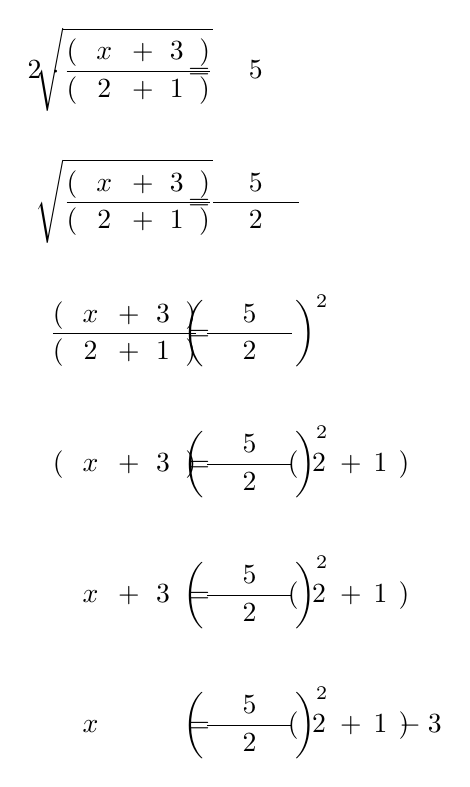
\begin{tikzpicture}[x=1em,y=-1em]
\node[anchor=base, inner sep=0pt] at (0.47,2.9) {$2$};
\node[anchor=base, inner sep=0pt] at (1.23,2.9) {$\cdot$};
\node[anchor=base, inner sep=0pt] at (3.72,2.9) {$\sqrt{\displaystyle\frac{\left(\pFourCell{1.94}{x}\pFourCell{0.84}{+}\pFourCell{1.62}{3}\right)}{\left(\pFourCell{1.94}{2}\pFourCell{0.84}{+}\pFourCell{1.62}{1}\right)}}$};
\node[anchor=base, inner sep=0pt] at (6.42,2.9) {$=$};
\node[anchor=base, inner sep=0pt] at (8.465,2.9) {$5$};
\node[anchor=base, inner sep=0pt] at (8.465,7.65) {$\displaystyle\frac{\pFourCell{3.09}{5}}{\pFourCell{3.09}{2}}$};
\node[anchor=base, inner sep=0pt] at (3.72,7.65) {$\sqrt{\displaystyle\frac{\left(\pFourCell{1.94}{x}\pFourCell{0.84}{+}\pFourCell{1.62}{3}\right)}{\left(\pFourCell{1.94}{2}\pFourCell{0.84}{+}\pFourCell{1.62}{1}\right)}}$};
\node[anchor=base, inner sep=0pt] at (6.42,7.65) {$=$};
\node[anchor=base, inner sep=0pt] at (3.72,12.385) {$\displaystyle\frac{\left(\pFourCell{1.94}{x}\pFourCell{0.84}{+}\pFourCell{1.62}{3}\right)}{\left(\pFourCell{1.94}{2}\pFourCell{0.84}{+}\pFourCell{1.62}{1}\right)}$};
\node[anchor=base, inner sep=0pt] at (6.42,12.385) {$=$};
\node[anchor=base, inner sep=0pt] at (8.465,12.385) {$\left(\displaystyle\frac{\pFourCell{3.09}{5}}{\pFourCell{3.09}{2}}\right)^{2}$};
\node[anchor=base, inner sep=0pt] at (3.72,17.105) {$\left(\pFourCell{1.94}{x}\pFourCell{0.84}{+}\pFourCell{1.62}{3}\right)$};
\node[anchor=base, inner sep=0pt] at (6.42,17.105) {$=$};
\node[anchor=base, inner sep=0pt] at (8.465,17.105) {$\left(\displaystyle\frac{\pFourCell{3.09}{5}}{\pFourCell{3.09}{2}}\right)^{2}$};
\node[anchor=base, inner sep=0pt] at (11.815,17.105) {$\left(\pFourCell{1.47}{2}\pFourCell{0.84}{+}\pFourCell{1.3}{1}\right)$};
\node[anchor=base, inner sep=0pt] at (2.49,21.825) {$x$};
\node[anchor=base, inner sep=0pt] at (3.88,21.825) {$+$};
\node[anchor=base, inner sep=0pt] at (5.11,21.825) {$3$};
\node[anchor=base, inner sep=0pt] at (6.42,21.825) {$=$};
\node[anchor=base, inner sep=0pt] at (8.465,21.825) {$\left(\displaystyle\frac{\pFourCell{3.09}{5}}{\pFourCell{3.09}{2}}\right)^{2}$};
\node[anchor=base, inner sep=0pt] at (11.815,21.825) {$\left(\pFourCell{1.47}{2}\pFourCell{0.84}{+}\pFourCell{1.3}{1}\right)$};
\node[anchor=base, inner sep=0pt] at (2.49,26.545) {$x$};
\node[anchor=base, inner sep=0pt] at (6.42,26.545) {$=$};
\node[anchor=base, inner sep=0pt] at (8.465,26.545) {$\left(\displaystyle\frac{\pFourCell{3.09}{5}}{\pFourCell{3.09}{2}}\right)^{2}$};
\node[anchor=base, inner sep=0pt] at (11.815,26.545) {$\left(\pFourCell{1.47}{2}\pFourCell{0.84}{+}\pFourCell{1.3}{1}\right)$};
\node[anchor=base, inner sep=0pt] at (14.04,26.545) {$-$};
\node[anchor=base, inner sep=0pt] at (14.93,26.545) {$3$};
\end{tikzpicture}
\end{center}

\newpage
\section*{Spaltentreue LaTeX-Ausgabe mit Spaltengrenzen}
\vspace{6mm}
\begin{center}
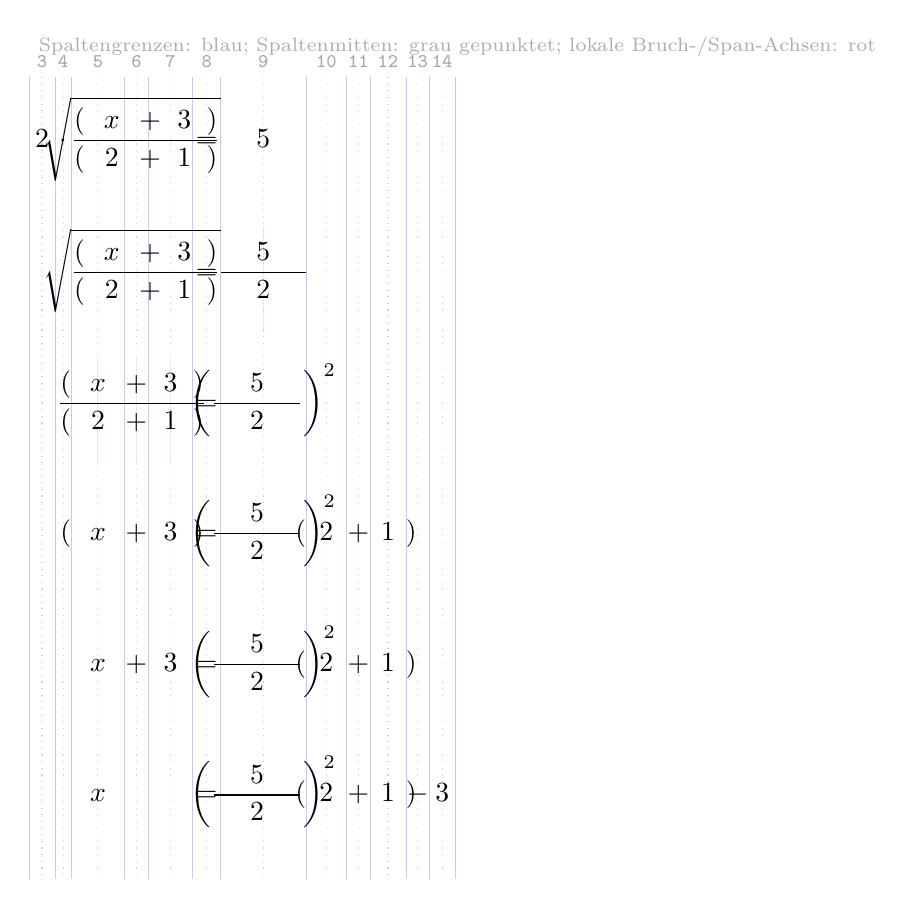
\begin{tikzpicture}[x=1em,y=-1em]
\node[font={\scriptsize}, text=gray!65, anchor=west] at (0,-0.75) {Spaltengrenzen: blau; Spaltenmitten: grau gepunktet; lokale Bruch-/Span-Achsen: rot};
\draw[blue!22, line width=0.28pt] (0,0.35) -- (0,29.33);
\draw[blue!22, line width=0.28pt] (0.94,0.35) -- (0.94,29.33);
\draw[blue!22, line width=0.28pt] (1.52,0.35) -- (1.52,29.33);
\draw[blue!22, line width=0.28pt] (3.46,0.35) -- (3.46,29.33);
\draw[blue!22, line width=0.28pt] (4.3,0.35) -- (4.3,29.33);
\draw[blue!22, line width=0.28pt] (5.92,0.35) -- (5.92,29.33);
\draw[blue!22, line width=0.28pt] (6.92,0.35) -- (6.92,29.33);
\draw[blue!22, line width=0.28pt] (10.01,0.35) -- (10.01,29.33);
\draw[blue!22, line width=0.28pt] (11.48,0.35) -- (11.48,29.33);
\draw[blue!22, line width=0.28pt] (12.32,0.35) -- (12.32,29.33);
\draw[blue!22, line width=0.28pt] (13.62,0.35) -- (13.62,29.33);
\draw[blue!22, line width=0.28pt] (14.46,0.35) -- (14.46,29.33);
\draw[blue!22, line width=0.28pt] (15.4,0.35) -- (15.4,29.33);
\draw[gray!35, dotted] (0.47,0.35) -- (0.47,29.33);
\node[font={\ttfamily\scriptsize}, text=gray!70, anchor=base] at (0.47,0) {3};
\draw[gray!35, dotted] (1.23,0.35) -- (1.23,29.33);
\node[font={\ttfamily\scriptsize}, text=gray!70, anchor=base] at (1.23,0) {4};
\draw[gray!35, dotted] (2.49,0.35) -- (2.49,29.33);
\node[font={\ttfamily\scriptsize}, text=gray!70, anchor=base] at (2.49,0) {5};
\draw[gray!35, dotted] (3.88,0.35) -- (3.88,29.33);
\node[font={\ttfamily\scriptsize}, text=gray!70, anchor=base] at (3.88,0) {6};
\draw[gray!35, dotted] (5.11,0.35) -- (5.11,29.33);
\node[font={\ttfamily\scriptsize}, text=gray!70, anchor=base] at (5.11,0) {7};
\draw[gray!35, dotted] (6.42,0.35) -- (6.42,29.33);
\node[font={\ttfamily\scriptsize}, text=gray!70, anchor=base] at (6.42,0) {8};
\draw[gray!35, dotted] (8.465,0.35) -- (8.465,29.33);
\node[font={\ttfamily\scriptsize}, text=gray!70, anchor=base] at (8.465,0) {9};
\draw[gray!35, dotted] (10.745,0.35) -- (10.745,29.33);
\node[font={\ttfamily\scriptsize}, text=gray!70, anchor=base] at (10.745,0) {10};
\draw[gray!35, dotted] (11.9,0.35) -- (11.9,29.33);
\node[font={\ttfamily\scriptsize}, text=gray!70, anchor=base] at (11.9,0) {11};
\draw[gray!35, dotted] (12.97,0.35) -- (12.97,29.33);
\node[font={\ttfamily\scriptsize}, text=gray!70, anchor=base] at (12.97,0) {12};
\draw[gray!35, dotted] (14.04,0.35) -- (14.04,29.33);
\node[font={\ttfamily\scriptsize}, text=gray!70, anchor=base] at (14.04,0) {13};
\draw[gray!35, dotted] (14.93,0.35) -- (14.93,29.33);
\node[font={\ttfamily\scriptsize}, text=gray!70, anchor=base] at (14.93,0) {14};
\node[anchor=base, inner sep=0pt] at (0.47,2.9) {$2$};
\node[anchor=base, inner sep=0pt] at (1.23,2.9) {$\cdot$};
\node[anchor=base, inner sep=0pt] at (3.72,2.9) {$\sqrt{\displaystyle\frac{\left(\pFourCell{1.94}{x}\pFourCell{0.84}{+}\pFourCell{1.62}{3}\right)}{\left(\pFourCell{1.94}{2}\pFourCell{0.84}{+}\pFourCell{1.62}{1}\right)}}$};
\node[anchor=base, inner sep=0pt] at (6.42,2.9) {$=$};
\node[anchor=base, inner sep=0pt] at (8.465,2.9) {$5$};
\draw[red!30, opacity=0.32, line width=0.35pt] (8.465,5.75) -- (8.465,9.55);
\node[anchor=base, inner sep=0pt] at (8.465,7.65) {$\displaystyle\frac{\pFourCell{3.09}{5}}{\pFourCell{3.09}{2}}$};
\node[anchor=base, inner sep=0pt] at (3.72,7.65) {$\sqrt{\displaystyle\frac{\left(\pFourCell{1.94}{x}\pFourCell{0.84}{+}\pFourCell{1.62}{3}\right)}{\left(\pFourCell{1.94}{2}\pFourCell{0.84}{+}\pFourCell{1.62}{1}\right)}}$};
\node[anchor=base, inner sep=0pt] at (6.42,7.65) {$=$};
\draw[red!30, opacity=0.32, line width=0.35pt] (2.49,10.5) -- (2.49,14.27);
\draw[red!30, opacity=0.32, line width=0.35pt] (3.88,10.5) -- (3.88,14.27);
\draw[red!30, opacity=0.32, line width=0.35pt] (5.11,10.5) -- (5.11,14.27);
\node[anchor=base, inner sep=0pt] at (3.72,12.385) {$\displaystyle\frac{\left(\pFourCell{1.94}{x}\pFourCell{0.84}{+}\pFourCell{1.62}{3}\right)}{\left(\pFourCell{1.94}{2}\pFourCell{0.84}{+}\pFourCell{1.62}{1}\right)}$};
\node[anchor=base, inner sep=0pt] at (6.42,12.385) {$=$};
\node[anchor=base, inner sep=0pt] at (8.465,12.385) {$\left(\displaystyle\frac{\pFourCell{3.09}{5}}{\pFourCell{3.09}{2}}\right)^{2}$};
\node[anchor=base, inner sep=0pt] at (3.72,17.105) {$\left(\pFourCell{1.94}{x}\pFourCell{0.84}{+}\pFourCell{1.62}{3}\right)$};
\node[anchor=base, inner sep=0pt] at (6.42,17.105) {$=$};
\node[anchor=base, inner sep=0pt] at (8.465,17.105) {$\left(\displaystyle\frac{\pFourCell{3.09}{5}}{\pFourCell{3.09}{2}}\right)^{2}$};
\node[anchor=base, inner sep=0pt] at (11.815,17.105) {$\left(\pFourCell{1.47}{2}\pFourCell{0.84}{+}\pFourCell{1.3}{1}\right)$};
\node[anchor=base, inner sep=0pt] at (2.49,21.825) {$x$};
\node[anchor=base, inner sep=0pt] at (3.88,21.825) {$+$};
\node[anchor=base, inner sep=0pt] at (5.11,21.825) {$3$};
\node[anchor=base, inner sep=0pt] at (6.42,21.825) {$=$};
\node[anchor=base, inner sep=0pt] at (8.465,21.825) {$\left(\displaystyle\frac{\pFourCell{3.09}{5}}{\pFourCell{3.09}{2}}\right)^{2}$};
\node[anchor=base, inner sep=0pt] at (11.815,21.825) {$\left(\pFourCell{1.47}{2}\pFourCell{0.84}{+}\pFourCell{1.3}{1}\right)$};
\node[anchor=base, inner sep=0pt] at (2.49,26.545) {$x$};
\node[anchor=base, inner sep=0pt] at (6.42,26.545) {$=$};
\node[anchor=base, inner sep=0pt] at (8.465,26.545) {$\left(\displaystyle\frac{\pFourCell{3.09}{5}}{\pFourCell{3.09}{2}}\right)^{2}$};
\node[anchor=base, inner sep=0pt] at (11.815,26.545) {$\left(\pFourCell{1.47}{2}\pFourCell{0.84}{+}\pFourCell{1.3}{1}\right)$};
\node[anchor=base, inner sep=0pt] at (14.04,26.545) {$-$};
\node[anchor=base, inner sep=0pt] at (14.93,26.545) {$3$};
\end{tikzpicture}
\end{center}
\end{document}
